\documentclass[a4paper,10pt]{book}
\usepackage{graphicx}
\usepackage{natbib}
\usepackage{amsmath}
\usepackage{amsfonts}
\usepackage{float}
\usepackage{caption}
\usepackage{wasysym}

\begin{document}
\begin{center}

\title{Discontinuous Galerkin reduced basis approximation for direct numerical simulation of the Navier Stokes equation: Master Thesis Report}


\author{Nirav Vasant Shah, \\M.Sc. Candidate, Water Resources Engineering and Management, \\University of Stuttgart, \\Stuttgart, Deutschland\\ 
\and Supervisor: Prof. Dr. Bernard Haasdonk,\\ Institute of Applied Analysis and Numerical Simulation, \\Universitity of Stuttgart,\\ Stuttgart, Deutschalnd\\ \and Co-advisor: Prof. Gianluigi Rozza,\\ Scuola Internazionale Superiore di Studi Avanzati, \\Trieste, Italy \\ \and Co-advisor: Dr. Martin Hess,\\ Scuola Internazionale Superiore di Studi Avanzati, \\Trieste, Italy }
\date{\today}
\maketitle

\end{center}

\tableofcontents






\chapter{Introduction}

The topic of the thesis deals with the reduced basis approach for the numerical solution of Navier Stokes Equation which is the core of Computational Fluid Dynamics. The thesis performs numerical simulation of Navier Stokes equation through Discontinuos Galerkin method and subsequently the parametrization of equation and reduced basis approach though Proper Orthogonal Decomposition.

The goal of thesis is to derive, discretize and implement the Discontinuous Galerkin weak form of Navier Stokes equation and perform numerical simulation of Navier Stokes equation. In the course of numerical solution we measure the simulation efforts.

Subsequently the equation is parametrized for parameters such as fluid property, geometry of domain, boundary condition. This allows the approximation of numerical solution, with approximation being with respect to parameter space. The solution of the parametrized form is stored for reduced basis evaluations.

The Proper Orthogonal Decompostion than sorts and extracts the stored  solutions based on eigen value. This extraction with parametrised form is used for prediction of full numerical solution. In this process the evaluations are made faster but with increase in induction of error. We compare the time saving vs. induced error.

In chapter 2, Navier Stokes equation is introduces. We first derive the Navier Stokes equation from conservation equation or Reynolds Transport Theoreom. We discuss about the flow classification and important issues related to numerical simulation of Navier Stokes equation. At the end of the chapter we discuss boundary conditions and its consequences on well posedness of the problem.

In chapter 3, we bring the problem from infinite dimensional domain to finite dimensional problem by introducing discretisation. We first introduce grid, constituents of elements and transformation between local and global geometry. Further the function spaces over the grid are discussed during which, the interpolation function, need for different function spaces for pressure and velocity is discussed. We than discuss the advantages of Discontinuous Galerkin method over Finite Volume method and develop more detailed understanding of the interpolation function used over the element. We further introduce the weak form and discrete formulation of Navier Stokes equation.

In chapter 4, We discuss implementation of the discrete form of Navier Stokes equation in RBMATLAB, an opensource software developed by University of Stuttgart and University of Münster, for numerical simulation. During the chapter we discuss matrix assembly, dimension of assembled matrices, solver performance issues, boundary treatment and basis function formation in RBMATLAB.

In chapter 5, we discuss some properties and tests useful for examination of assembled matrices. We further present results from numerical experiment and some case studies.

In chapter 6, we interpret and explain the outcomes of numerical experiments. 

In chapter 7, we introduce parametric space, discuss parametrization and empirical interpolation method. We than perform reduced basis approximation and proper orthogonal decomposition method. 

In chapter 8, we perform the numerical experiment related to reduced order modelling and discuss, interpret and assess the results form reduced basis method.

In appendix, supplementary theoretical background is provided which is expected to help the readers to better comprehend the thesis.

\newpage


\chapter{Engineering perspective and mathematical formulation} 

The subject of mathematical applications in fluid mechanics starts with  one of the variants of Navier Stokes equation. Almost all processes of fluid mechanics require considerations related to Navier Stokes equation. Hence the importance of Navier Stokes equation is impossible to be ignored as far as mathematical approaches in fluid mechanics are concerned. The numerical method for incompressible equation is far more simple as compared to compressible Navier Stokes equation. This is due to removal of dependence on equation of state. 

\section{Derivation of Navier Stokes equation}

Before deriving Navier Stokes equation we introduce some notations. The domain is denoted by $\Omega \subseteq \mathbb{R}^d $. The domain boundary is denoted by $\Gamma$. The domain boundary is divided into Dirichlet boundary $\Gamma_D$ and Neumann boundary $\Gamma_N$ i.e. $\Gamma_D \cup \Gamma_N = \Gamma $. 

The governing equations for incompressible stokes flow are conservation equations: Mass conservation and momentum conservation. The cnoservations equations are derived based on concept of control volume and control surface. Control volume is the volume, fixed or moving with constant velocity in space, through which fluid moves. Control surface is the surface enclosing control volume. All equations can be derived from Reynold's transport equation:


\begin{equation} \label{rtt} 
\frac{dB}{dt}|_{cs} = \frac{d}{dt} \int_{cv} b \rho dV + \int_{cs} b \rho u.dA 
\end{equation}

\begin{center}
$cv$ = Control volume\\
$cs$ = Control surface\\
$B$ = Extensive property under consideration  \\
$b$ = Intensive property corressponding to B \\
$\rho$ = Density of fluid \\
$u$ = Velocity of fluid at the control surface \\
\end{center}

If in the above equation $B$ is substituted as momentum $P$, correspondingly $b$ as velocity $u$, we receive change in momentum which as per Newton's Second law of Motion is equal to sum of external forces acting on the system. 

\begin{equation}\label{External force lhs}
F = \frac{dP}{dt} = \frac{d}{dt} \int_{cv} u \rho dV + \int_{cs} u \rho u.dA 
\end{equation}

This sum of forces arises from stresses $\sigma$ (shear stresses and normal stresses) and external force $f$ such as weight, Electromagnetic force. 

\begin{equation}\label{External force rhs}
F = \int_{cs} \sigma \cdot dA + \int_{cv} \rho f dV
\end{equation}

Where,\\
$\sigma =$ Stress\\
$f =$ External force per unit volume\\

Equating external force with change in momentum i.e. equating \eqref{External force lhs} and \eqref{External force rhs} and with the application of Gauss divergence theoreom we derive Navier Stokes equation, 

\begin{equation} \label{navier_stokes}
-2\nabla \cdot (\nu \nabla^s u) + (1/\rho) \nabla p + (u \cdot \nabla)u = f \quad   \textnormal{in}  \quad \Omega
\end{equation} 

The incompressible mass conservation equation can be written as
\begin{equation}\label{mass_conservation}
\nabla \cdot u=0 \quad   \textnormal{in}  \quad \Omega
\end{equation}

The boundary conditions can be expressed as,

Dirichlet boundary:
\begin{equation}\label{dirichlet_ns}
u=u_D \quad \textnormal{on} \quad \Gamma_D
\end{equation}

Neumann boundary:
\begin{equation} \label{neumann_ns}
-pn + 2\nu(n \cdot \nabla^s)u = g \quad   \textnormal{on}  \quad \Gamma_N
\end{equation}

Where,\\
$u$ = flow velocity and $u:\Omega \rightarrow \mathbb{R}^d$ \\
$p$ = pressure and $p:\Omega \rightarrow \mathbb{R}$\\
$\nu$ and $\rho$ = kinematic viscocity and density (fluid properties) and $\nu:\Omega \rightarrow \mathbb{R}$ and $\rho:\Omega \rightarrow \mathbb{R}$\\
$f$ = external force $f:\Omega \rightarrow \mathbb{R}^d$\\
$u_D$ = specified flow velocity at Dirichlet boundary $u_D:\partial \Omega_D \rightarrow \mathbb{R}^d$\\
$n$ = normal unit vector $n:\partial \Omega \rightarrow \mathbb{R}^d$\\
$g$ = specified Neumann flux $g:\partial \Omega_{N} \rightarrow \mathbb{R}^d$\\

The \eqref{navier_stokes} is known as Strong form.

It can be seen that the steady state Navier Stokes equation is non linear and has two unknown variables, pressure $P$  and velocity $u$. The additional equation added by continuity equation is hence necessary in order to sufficient number of equation for sufficient number of unknowns.

We also introduce dimensionless number Reynolds number,$Re$ which is the most characteristic of the flow. Reynolds number is defined as the ratio of Inertial force to the viscous force and is measured by,
\begin{equation} \label{reynolds_number}
Re =  u L / \nu
\end{equation}

Here, $L$ = Characteristic geometrical dimension, for example Diameter of Pipe in case of pipe flow or Span of wing of Aircraft in case of flow over aircraft wing\\

\subsection{Direct numerical simulation} 

We now differentiate between the type of flows, Laminar and Turbulent.\\
Laminar flow is characterised by well defined velocity and pressure field and low Reynolds number. This flow has very low velocity and pressure fluctuations. The viscous force is balanced by pressure force and the flow has negligible inertial force. Mathematically, the non linear term in \eqref{navier_stokes} is no longer present. Such equation is known as Stokes equation.\\

In contrast, the Turbulent flow is characterised by fluctuations in velocity and pressure field and high Reynolds number. The flow has high velocity and inertial force is present in addition to viscous and pressure force. This inertial force makes the equation \eqref{navier_stokes} non linear. The fluctuations of velocity and pressure are of the order of Kolmogrov scale.

The method used for solving equation \eqref{navier_stokes} numerically is known as Direct Numerical Simulation, abbreviated as DNS. The direct numerical simulation could be computationally very expensive especially in applications such as turbulent flows as the time and space grid size is of the order of Kolmogrov scale but the time period or space dimension over which the simulation is carried out are very large. In order to avoid such computational expenses alternate models are used replacing original model. However, the alternate model can not explain completely the flow physics. The prediction of accurate flow physics description requires economical numerical solution of \eqref{navier_stokes}. It is to be noted that simulation of turbulent flow is always a compromise between required flow physics prediction and computational efforts.

\section{Wellposedness of strong form of Navier Stokes equation}

\chapter{Discretization and function spaces}
\section{Grid geometry}

In numerical anlysis the problem is solved into finite dimensional domain. This finite dimensional domain is constructed by projecting actual domain onto a subdomain called as grid through a grid function.
If the original domain is denoted by $\Omega$ we denote the grid by $\Omega_h$ and define grid function by $G:\Omega \rightarrow \Omega_h$ and we note that $\Omega_h \subset \Omega$. In present case we use triangular grid and denote each triangle as $\tau_h$. We also note that $\Omega_h = \cup_{h=1}^{nel} \tau_h$ where $nel$ is the total number of elements in the grid. Each triangle is an 'Element'of the grid. The boundary betwen elements i.e. interelement boundary is denoted by $\Gamma$. In case of grid the boundaries comprises domain boundaries and interelement boundaries i.e. $\partial \Omega = \Gamma_D \cup \Gamma_N \cup \Gamma$. During discussion on jump operator and average we denote the element under consideration as $\tau_{h}^-$ and neighbouring element as $\tau_{h}^+$. We also denote normal pointing from element itself towards neighbouring element as $n^+$ and normal pointing from neighbouring element towards element itself as $n^-$. Corresspondingly every quantity from element itself is denoted by superscript $+$ and from neighbouring element is denoted by $-$.

In case of 2-dimensional domain the grid could be triangular grid or rectangular grid. The triangular grids are useful for irregular geometry and also on regular geometry if flow physics, and correspondigly the solution, is expected to be complex. This flexibility requires additional efforts to define the grid accurately. That is, unlike structured grid, an unstructured grid needs to define connectivity of vertices, which form an edge, which in turn forms a face. These faces in case of 3-dimensional grid constitute a tetrahedral elements. In case of 2-dimensional grids we have only faces which are 2-dimensional entity, edges which are 1-dimensional entity and points or vertices which are 0-dimensional entities.

For triangular grids we also consider Barycentric co-ordinate system. In Barycentric co-ordinate system any point within the triangle is reprensented in terms of vertices forming the triangle. Any point $r$ within triangle is expressed in terms of vertices forming the triangle $r_1,r_2,r_3$. This is represented as,

\begin{equation}\label{barycentric point}
r = \lambda_1 r_1 + \lambda_2 r_2 + \lambda_3 r_3
\end{equation}

where, $\lambda_1, \lambda_2, \lambda_3$ are weightages which represent the distance of point $r$ from respective vertices. The weightages satisfy the criteria,

\begin{equation}\label{lambda constraint}
\lambda_1 + \lambda_2 + \lambda_3 = 1
\end{equation}

Hence we only need to satisfy 2 values in 2-dimensional plane in order to fully define the position of point.

For example, the centroid of triangle will have $\lambda_1 = 1/3, \lambda_2 = 1/3$. By \eqref{lambda constraint} we have $\lambda_3=1/3$ i.e. a point which is equidistant to all vertices.

\section{Grid parameters}

We refer "Grid parameters" as the geometrical parmeters which are dependent only on the geometry of the problem or the grid or both. These parameters do not depend upon the mathematical formulation but are supplementry to the mathematical formulation. On the triangular grid we have 3 entities faces, edges, vertices as explained above. From faces we have the area (equivalent to volume of element in case of 3-dimensional grid) and Jacobian. As explained later in the weak form of Navier Stokes Compact Discontinuous Galerkin and transformation between local and global geometry the area of element is useful for volume intergral terms and the Jacobian is useful for gradient transformation. From edges we derive the edge length which is useful for boundary integral terms and normal vector which is useful for flux calculation. The normal vector is considered positive when pointing outward from the element negative when pointing inward to the element. Every element has 3 neighbouring element and the element shares each of his edge with one of its neighbour. From vertices we derive the vertex index which helps to define the connectivity of the vertices which is useful especially in case of unstructured grid. 

In order to give clear visualization of domain or precisely, continuous domain and grid or discretiozed domain we introduce a unit square with circular obstacle with center of circle coinciding with center of square. 

\newpage

\begin{figure}
  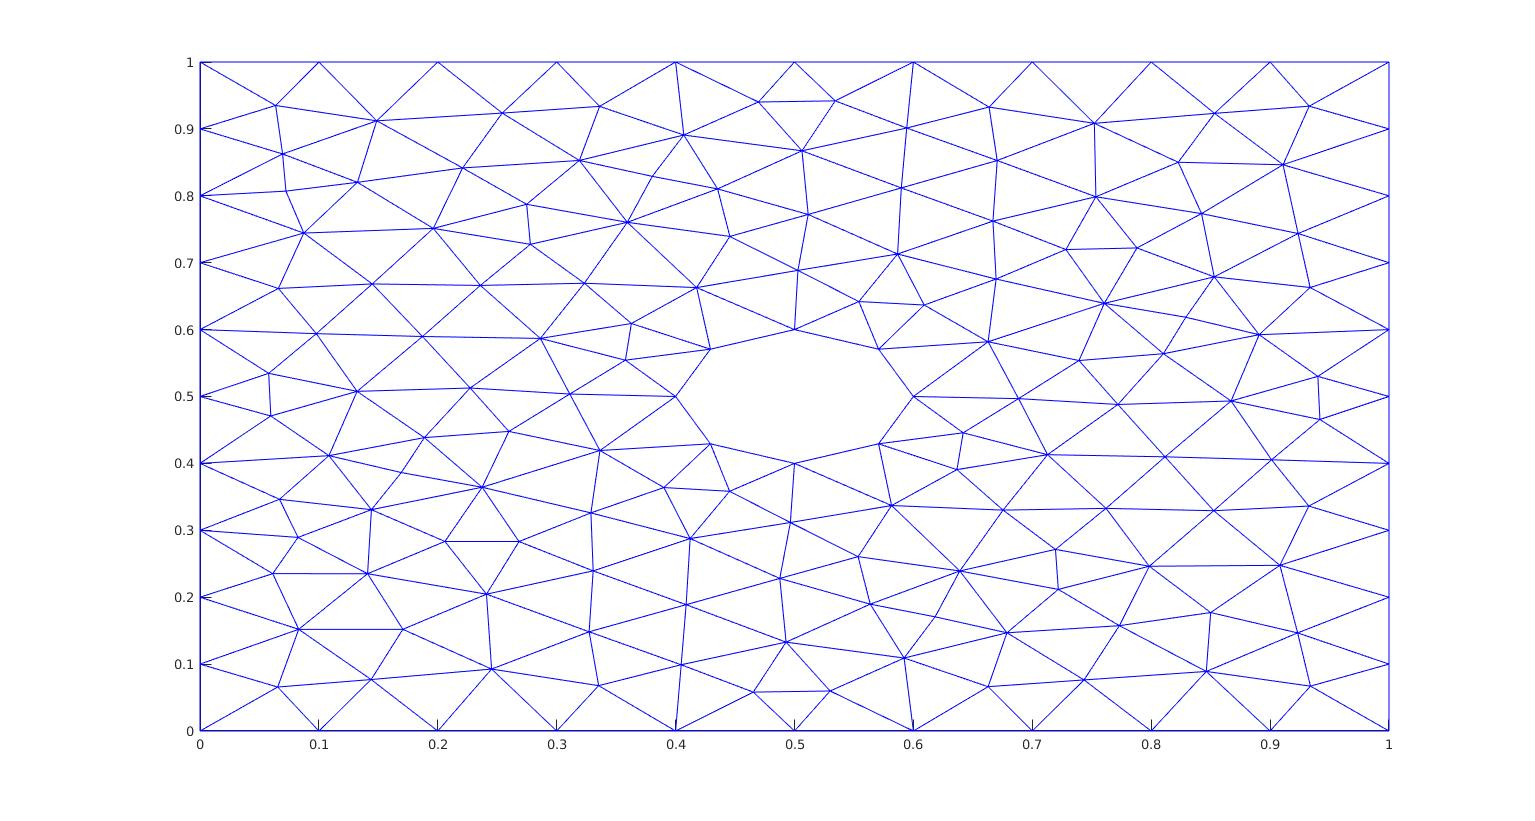
\includegraphics[width=\linewidth,scale=0.5]{grid.jpg}
  \caption{Discretized domain or grid}
  \label{fig:Mesh}
\end{figure}

\begin{figure}
  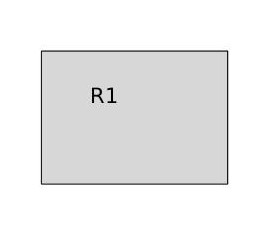
\includegraphics[width=\linewidth,scale=0.5]{domain.jpg}
  \caption{Continuous domain}
  \label{fig:Domain}
\end{figure}

\newpage
\newpage

\section{Global and local co-ordinate system}

The integral terms are evaluated on a reference triangle instead of element itself. Accordingly, a co-ordinate transformation is performed for every element to reference triangle for evaluating integrals. The co-ordinate system in which reference triangle lies is called reference or local co-ordinate system and the co-ordinate system in which element itself lies is called global co-ordinate system. The reference triangle has vertices $(0,0),(1,0),(0,1)$ in order. The element is defined by vertex indices in order forming triangle. The mapping from reference triangle $\hat{T}$ to each element $\tau_k$ is defined by mapping,

\begin{equation}\label{local global mapping}
F_k:\hat{T} \rightarrow \tau_k
\end{equation}

This mapping function is defined as,

\begin{equation}\label{local global mapping equation}
F_k: X = J_k \hat{X} + C
\end{equation}

Here,

$J_k$ = Jacobian matrix of element $k$ or Rotational matrix for transformation from local co-ordinate system to global co-ordinate system\\
$C$ = Translational matrix for transformation from local co-ordinate system to global co-ordinate system\\
$X$ = Co-ordinates of vertices of element in Global co-ordinate system\\
$\hat{X}$ = Co-ordinates of vertices of reference triangle in local co-ordinate system\\


We consider image of global function space on reference triangle and is represented by superscript $\hat{•}$. This function space is known as local basis function space. 

\begin{picture}(300,100)(0,0) 
\put(0,0){\line(1,0){50}}
\put(50,0){\line(1,1){100}}
\put(0,0){\line(3,2){150}}
\put(200,0){\line(1,0){100}}
\put(300,0){\line(-1,1){100}}
\put(200,100){\line(0,-1){100}}
\end{picture}

\begin{center}
Global geometry (left) to Local geometry (right)
\end{center}

The volume integral of function $f(x)$ in global geometry is related to volume integral on local geometry as 
\begin{equation}\label{integral_local_global_volume}
\int_\Omega f(x) dx = \sum_{k=1}^{nel} \int_{\tau_k} f(x) dx = \sum_{k=1}^{nel} \int_{\hat{T}} f(\hat{x}) \det(J_k) d \hat{x}
\end{equation}

The linear boundary integral of function $f(x)$ on global geometry is related to boundary integral on local geometry as, 
\begin{equation}\label{integral_local_global_boundary}
\int_{\partial\Omega} f(x) ds = \int_{\partial\hat{\Omega}} f(\hat{x}) l d \hat{s}
\end{equation}

Also, the following holds,
\begin{equation}\label{derivative_transformation}
\nabla g = JIT * \hat{\nabla} \hat{g}
\end{equation}


where, \\

$l$ = length of boundary on global geometry\\
$g$  = A function in global co-ordinate system\\
$\hat{g}$  = A function in local co-ordinate system corresponding to function in $g$ in global co-rodinate system\\

Here $g$ and $\hat{g}$ satisfy,
\begin{equation}\label{func_transformation}
g(x) = \hat{g}(\hat{x})
\end{equation}

\subsection{Jump operator}

The jump operator of quantity u at an internal boundary is defined as,
\begin{equation}\label{jump operator}
[u]=u^+ \cdot n^+ + u^- \cdot n^-
\end{equation}

where n is normal to the cell boundary pointing outwards from the cell.

As pointed out by \cite{Montlaur2} this jump has two disadvantages.

1. The function space of quantity itself and the function space of jump are diferrent that is, jump of vector is scalar and jump of scalar is vector.\\
2. The use of this definition camoulages the presence of normal.

To overcome this disadvantages \citep{Montlaur2} used the jump definitions as ,

(here, Subscript i referes to the elements itself and subscript j refers to the neoghbouring element, $[[ ]]$ refers to jump and n refers to normal vector.)

1. \\
$[[pn]] = p^+ n^+ + p^- n^- $ on $\Gamma$\\
$[[pn]] = p n $ on $\Gamma_D$\\
where $p$ is scalar. \\

2. \\
$[[n \otimes v]] = n^+ \otimes v^+ + n^- \otimes v^-$ on $\Gamma$\\
$[[n \otimes v]] = n \otimes v$ on $\Gamma_D$\\
 or \\
$[[n \cdot v]] = n^+ \cdot v^+ + n^- \cdot v^-$ on $\Gamma$\\
$[[n \cdot v]] = n \cdot v$ on $\Gamma_D$\\
where $v$ is vector\\

3. \\
$[[n \cdot \sigma]] = n^+ \cdot \sigma^+ + n^- \cdot \sigma^-$ on $\Gamma$\\
$[[n \cdot \sigma]] = n \cdot \sigma$ on $\Gamma_D$\\
where $\sigma$ is Second order vector

\subsection{Average operator}

Similarly the average operator is defined as,

\begin{equation}\label{average operator}
\left\lbrace u \right\rbrace = \frac{u^+ + u^-}{2}  
\end{equation} 

\section{Discontinuous Galerkin Method}

In the context of discontinuous galerkin method we introduce function space $V$($\tau_h$) and $Q$($\tau_h$) for analytical solution of velocity and analytical solution of pressure respectively. The space containing high fidelity solution is called truth space denoted by $V_h$. The dimension of $V_h$ is denoted as $N_h$. (The subscript h hereafter refers to truth space.)

\begin{equation} \label{velocity_test}
V = \lbrace \phi \in L^2(\Omega)| v|_k \in P^D(K) \forall K \in \tau_h \rbrace
\end{equation}

\begin{equation} \label{pressure_test}
Q = \lbrace \psi \in L^2(\Omega)| q|_k \in P^{D-1}(K) \forall K \in \tau_h \rbrace
\end{equation}

Here, $P^D$ denotes space of polynomials of degree at most $D$ over $\Omega$.

We apply similar procedure as in Finite element method i.e. multiplying the partial differential equation by test function and intergration by parts. However, we note that our test function is not continuous on the interface. Hence, we require flux approximations and jumps at the interface. These requirements have given rise to different discontinuous Galerkin methods. For explanation of each method we refer to literatures such as \cite{persson} for local discontinuous galerkin and \cite{Montlaur} for Compact discontinuous Galerkin and Interior penalty method. 

Discontinuous Galerkin methods for Navier Stokes equation were compared by \cite{Montlaur}. The local discontinuous Galerkin(LDG) method extends the computational stencil beyond immediate neighbours whereas compact discontinuous Galerkin(CDG) and interior penalty method(IPM) only connect to neighbouring elements. The CDG method provides more flexibility with respect to stabilisation constant at the cost of additional simulation effort related to computation of lifting operator, while the IPM method requires restrictions on penalty parameter in order to maintain coercivity of bilinear form. Both methods, CDG and IPM, have almost similar convergence rates. 

\subsection{Nodal basis function and Orthonormal basis function}

The "Basis function" are also known as "Interpolation function" or "Ansatz function". There are two kinds of basis function which are used in the application of Finite element or Discontinuous Galerkin Method. 
Before, explaining the diferrence between two types of basis functions, we understand the procedure to define the function completely. \\

In order to define a polynomial of given degree completely, we need to calculate its co-efficients. A polynomial of degree n in 1-dimensional domain has $n+1$ coefficients. In case of 2-dimensional domain the number of co-efficients become $(n+1)(n+2)/2$. Two define these co-efficients the known values of function at number of points equal to the number of co-efficients is required. These points are known as nodes. In case of triangular element, the nodes located as,\\

1. For polynomial of degree 1 i.e. $p=1$, the nodes are selected as vertices of element.\\
2. For polynomial of degree 2 i.e. $p=2$, the nodes are selected as vertices of element and mid point of edges.\\

\begin{figure}
  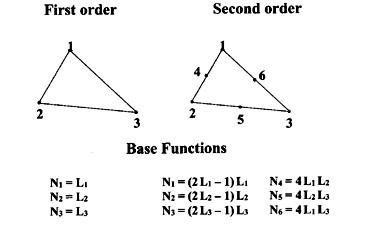
\includegraphics[width=\linewidth]{fem_triangle.jpg}
  \caption{Finite Element nodes on triangle for $p=1$ and $p=2$ \cite{plasma}}
  \label{fig:Nodes on Triangular Element}
\end{figure}

Similarly for higher order polynomial the nodes are selected as shown in \ref{fig:Nodes on Triangular Element}.

\begin{figure}
  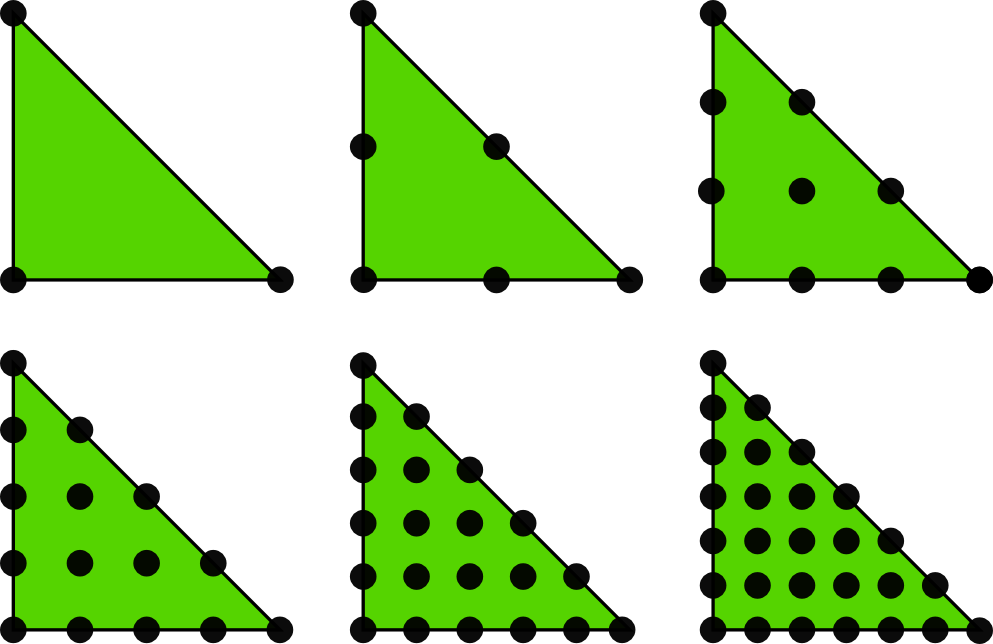
\includegraphics[width=\linewidth]{fem_triangle_2.png}
  \caption{Finite Element nodes on triangle for polynomials of different degrees \\ http://hplgit.github.io/INF5620/doc/pub/sphinx-fem/.\_main\_fem009.html}
  \label{fig:Nodes on Triangular Element}
\end{figure}

\subsection{Nodal Basis Function}

Nodal basis function is also known as "Shape function". This basis function has value of 1 at its respetive node and 0 at other nodes. At all other points it is interpolated based on the degree of the basis function. 

\subsection{Orthonormal Basis Function}

Orthonormal basis functions are the basis functions defined in such a way that all basis functions are orthonormal to each other. The number of orthonormal basis functions for a given element is same as number of Nodal basis functions. In fact, in present analysis the orthonormal basis functions are derived from Nodal basis functions.

\newpage
\section{Weak and discrete form of Navier Stokes equation}

Following the approach presented by \cite{Montlaur} and \cite{Montlaur2} we arrive at weak form of Navier Stokes interior penalty approximation as,

\begin{equation}\label{Navier Stokes weak form}
a_{IP}(u,\phi)+c(u : u, \phi) + b(\phi , p) + ({p},[n \cdot \phi])_{\Gamma \cup \Gamma_D} = l_{IP}(\phi)
\end{equation}

\begin{equation}\label{aIP}
a_{IP} = (2\nu \nabla^s u,\nabla^s \phi) + C_{11}([n \otimes u],[n \otimes u])_{\Gamma \cup \Gamma_D} - (2 \nu {\nabla^s u},[n \otimes \phi])_{\Gamma \cup \Gamma_D} - (2 \nu [n \otimes u], {\nabla^s \phi})_{\Gamma \cup \Gamma_D} 
\end{equation}

\begin{equation}\label{lIP}
l_{IP}(\phi) = (f,\phi) + (t,\phi)_{\Gamma_N} + C_{11}(u_D,\phi)_{\Gamma_D} - (n \otimes u_D, 2 \nu \nabla^s \phi)_{\Gamma_D}
\end{equation}

\begin{equation}\label{b_continuity}
b(\phi,p) = -\int_{\Omega} \psi \nabla \cdot \phi
\end{equation}

Here, $c(u : u, \phi)$ is non linear term which we discuss later.

Following discretization of the continuous form we arrive at discrete form as below. We refer hereafter, throughout thesis, subscript $h$ for function in discrete form.

\begin{equation}\label{Navier Stokes Matrix form}
A U + B P = F
\end{equation}

where,\\
$A$ and $B$ = Stiffness matrix\\
$U$ = Global velocity degree of freedom vector\\
$P$ = Global pressure degree of freedom vector\\
$F$ = Right hand side vector\\

\section{Coercivity of bilinear form} 

For the term $a_{IP}$ which has elliptic behavior we discuss now coercivity, continuity and inf-sup condition\cite{riviere}.


A bilinear form $a(u,v)$ is said to be coercive if there exists a constant $c_{11} > 0$ such that

\begin{equation}\label{Coercivity}
a(v,v) > c_{11} ||v||^2   \exists   c_{11} > 0
\end{equation}

Based on \ref{basics}
\begin{equation}\label{Coercivity_constant}
a(v,v) \geq (1-\frac{\delta}{2} |1-\epsilon|) \Sigma_{E \epsilon \varepsilon_h} ||\nu^{1/2} \nabla v ||^2_{L^2(E)} + \Sigma_{e \epsilon \Gamma_h \cup \Gamma_D} \frac{\sigma_e^0 - \frac{C_t^2 \nu_1^2 n_0}{2 \delta K_0}|1-\epsilon|}{|e|^{\beta_0}} ||[v]||^2_{L^2(e)}
\end{equation}

\section{Continuity of bilinear form}

A bilinear form $a(u,v)$ is said to be continuous if there exists a constant $\Gamma > 0$ such that

\begin{equation}\label{Continuity}
a(u,v) \leq \Gamma ||u||||v||   \exists   \Gamma > 0
\end{equation}


\begin{equation}\label{Continuity_constant}
\begin{Huge}
\Gamma CONSTANT AND DERIVATION
\end{Huge}
\end{equation}

\section{Inf-sup contdition}

For the stability of non-coercive problem the inf-sup condition is important which is stated as, \cite{crbm} 

\begin{equation}
\exists \beta > 0 : \beta(\mu) = inf v \epsilon V \ {0}  sup w \epsilon W \ {0} \frac{a(v,w;\mu)}{||v||_{\mathbb{V}} ||w||_{\mathbb{W}} } \geq \beta \forall \mu \epsilon \mathbb{P}
\end{equation}



\chapter{Implementation aspects}

We discuss now the implementation of discrete formulation of Navier Stokes Discontinuous Galerkin weak formulation in RBMATLAB, A MATLAB library containing all our reduced simulation approaches for linear and nonlinear, affine or arbitrarily parameter dependent evolution problems with finite element, finite volume or local discontinuous Galerkin discretizations. 

Before we discuss details of implementation it is important to understand some frequently used terminologies and the data type of Basis Function and derivative of basis function in RBMATLAB.

\section{Terminologies}


A. $params$ and $paramsP$ : $params$ and $paramsP$ are structures corressponding to velocity and pressure respective containing following fields\\

1. $dimrange$ : We refer $dimrange$ as dimension of range or solution. In present analysis this means Velocity has $dimrange$ of 2 and Pressure has $dimrange$ of 1.\\

2. $pdeg$ : We refer $pdeg$ as the degree of polynomial used as interpolation polynomial.\\

3. $ndofs\_per\_element$ : We refer $ndofs\_per\_element$ as the number of degrees of freedom over an element. \\

B. $grid$ : $grid$ is the structure containing following fields\\

4. $nelements$ : $nelements$ is total number of elements in grid.\\

5. $NBI$ : $NBI(i,j)$ represents element number of $j$th neighbour of element $i$. 1$\leq i \leq nelements$ and 1$\leq j \leq$3.\\

6. $NX$ and $NY$ : $NX(i,j)$ and $NY(i,j)$ represent x component and y component of normal from  element $i$ to $j$ numbered neighbour.\\

7. $JIT$ : $[JIT(k,:,1)',JIT(k,:,2)']$ represents Jacobian Inverse Transpose of element $k$.\\

8. $A$ : $A(k)$ represents area of $k$th element.\\

9. $EL$ : $EL(i,j)$ represents length of edge between element $i$ and $j$th neighbour of Element $i$. The notation $EL$ is used when $i$ refers to superscript $+$ and $j$ refers to element with superscript $-$.\\

We also use some other local variables as below:

10. $k$ : $k$ represents the element number and 1$\leq k \leq nelements$.\\

11. $ids$ : $ids(i,:)$ represents the indices of degree of freedom of element $i$ where 1$\leq i \leq nelements$ in global degree of fredom vector. Size of $ids(i,:)$ is $ndofs\_per\_element$. $ids\_velocity$ corressponds to indices corressponding to velocity and $ids\_pressure$ corressponds to indices corressponding to pressure. Further notations such as $ids\_velocity\_neighbour$ should be read as $ids$ of velocity degree of freedom of neighbouring element.\\

Basis Function $\phi_h$ in RBMATLAB :\\

The Basis functions in RBMATLAB is generated by routine called ldg\_evaluate\_basis.m.\\

We interpolate the solution from solution at known degrees of freedom. In matrix formulation this means basis function is matrix of the size,

\begin{equation}\label{basis_func_rbmatlab}
\phi_h \epsilon \mathbb{R}^{ndofs\_per\_element X dimrange}
\end{equation}

where each row of $\phi_h$ denotes 

This representation creates many zeros in matrix, however, it does not require new evaluation for each component of vector quantity in dimrange of solution.

Due to the zeros in the basis function, zeros in derivative of basis functions are produced. 

The derivative of basis function is generated by routine ldg\_evaluate\_basis\_derivative. The derivative of basis function $(\phi_h)_{i}$, where 1$\leq i \leq nodfs\_per\_element$ is a cell containing matrix $\nabla (\phi_h)_{i}$ of size,
\begin{equation}\label{basis_func_derivative_rbmatlab}
\nabla (\phi_h)_{i} \epsilon \mathbb{R}^{{dimrange} X 2}
\end{equation}

where the colmuns of matrix corresspond to $\nabla_x (\phi_h)_{i}$ and $\nabla_y (\phi_h)_{i}$ .

\section{Assembly of average operator}

Average of quantity, $A_h$ in discrete form is assembled as,

\begin{equation}\label{Average operator}
{A_h} = (A_h^+ + A_h^-)/2
\end{equation}

The assembly of average operator is relatively simple as compared to jump operator which is explained in section \ref{Jump operator}

\section{Jump operator} \label{Jump operator}

Jump of quantity, $A_h$ in discrete form is assembled as,
\begin{equation} \label{Jump_operator}
[A_h] = A_h^+ n^+ + A_h^- n^-
\end{equation}

In case of terms such as $[A_h],[B_h]$ we assemble matrices as, 

For internal edges $\Gamma$,

\begin{equation} \label{Jump operator L2}
[A_h],[B_h] = A_h^+ n^+ B_h^+ n^+ + A_h^+ n^+ B_h^- n^- + A_h^- n^- B_h^+ n^+ + A_h^- n^- B_h^- n^-
\end{equation}

and for dirichlet edges $\Gamma_D$

\begin{equation} \label{Jump operator L2 for dirichlet}
[A_h],[B_h] = A_h^+ n^+ B_h^+ n^+ 
\end{equation}


\subsection{Matrix assemblies}

We repeat here, for conveniece, again notations of $L^2$ scalar product from weak form

Here, $(p,q)$ refers to,

If $p$ and $q$ are scalars,
\begin{equation}\label{inner product scalars}
(p,q)=\int_{\Omega} pq d \Omega 
\end{equation}

If $p$ and $q$ are vectors,
\begin{equation}\label{Inner product vectors}
(p,q)=\int_{\Omega} p \cdot q d\Omega
\end{equation}

If $p$ and $q$ are tensors,
\begin{equation}\label{Inner product tensors}
(p,q)=\int_{\Omega} p:q d\Omega
\end{equation}

i.e. (.,.) denotes $L_2$ inner product.

The matrices from weak form of Navier Stokes equation have been assembled in 3 steps,

1. Evaluating function at vertex of local element and transform to global geometry\\
2. Performing integral of function over local element and transform to global geometry(if not done in step 1)\\
3. Performing a loop over all elements and allocate integral at position in global matrix(for bilinear terms)/global vector(for linear terms) according to index of element degree of freedom in global degree of freedom vector.

We also perform numerical integration over domain $\Omega$ as,

\begin{equation}\label{numerical integration}
\int_{\Omega} f(x) = \Sigma_{i=1}^{nop} f(x_i) * w_i
\end{equation}

Where, \\

$x_i$ = Location of function evaluation
$w_i$ = Weight at corressponding point
$nop$ = Number of points

The location of function evaluation, number of points and weights are based on Gaussian quadrature rule.

Also the determinant of jacobian is twice the area of triangle.

\begin{equation}\label{determinant to area}
J(k) = 2*A(k)
\end{equation}

With this preliminary informations we discuss now the assembly of matrices.

1. $(\nabla \phi, \nabla \phi)$:\\

Step 1: Evalauation of $(\nabla \phi , \nabla \phi)$,

We first evaluate derivative of $\hat{\phi}$ and $JIT(k,:,:)$ through ldg\_evaluate\_basis\_derivative and grid structure. We also perform elementary operation so as to rceiv one global basis function in each row. The matrix transformation from local derivative to global derivative is based on the formula \ref{derivative_transformation}.

We than assemble matrix $res_1[i,j]=\phi_i*\phi_j^T$ for $1 \leq i,j \leq ndofs\_per\_element$\\

Step 2: Performing integration in global co-ordinate system,

We perform the numerical integration as per \ref{numerical integration} 

$res_2 = \int_{\hat{\Omega}} res_1 *2*grid.A(k)  d \hat{\Omega}$\\

Step 3: Looping over each element and performing following operation in each loop $res_3[ids\_velocity,ids\_velocity]=res_2$\\


2. $([n \otimes \phi_h], [n \otimes \phi_h])_{\Gamma \cup \Gamma_D}$ :

Step 1: On local element following functions are evaluated,\\
\\
$res_1^{++} = [n \otimes \hat{\phi_h]}^+ [n \otimes \hat{\phi_h}]^+$\\
$res_1^{+-} = [n \otimes \hat{\phi_h}]^+ [n \otimes \hat{\phi_h}]^-$\\
$res_1^{-+} = [n \otimes \hat{\phi_h}]^- [n \otimes \hat{\phi_h}]^+$\\
$res_1^{--} = [n \otimes \hat{\phi_h}]^- [n \otimes \hat{\phi_h}]^-$\\

Please note that $\hat{\phi_h}$ is evaluated at local coordinate corressponding to global coordinate.

Step 2: In step 2 we perform following integration, 
We perform the numerical integration as per \ref{integral_local_global_boundary}
\\ 
$res_2^{++} = \int_{\Gamma} res_1^{++} * grid.EL$\\
$res_2^{+-} = \int_{\Gamma} res_1^{+-} * grid.EL$\\
$res_2^{-+} = \int_{\Gamma} res_1^{-+} * grid.EL$\\
$res_2^{--} = \int_{\Gamma} res_1^{--} * grid.EL$\\

Step 3: Loop over all elements, define the global assembly matrix as zero matrix and perform following operation in each loop,
\\
$res_3^{++}[ids\_velocity\_self,ids\_velocity\_self] = res_2^{++}$\\
$res_3^{+-}[ids\_velocity\_self,ids\_velocity\_neighbour] = res_2^{+-}$\\
$res_3^{-+}[ids\_velocity\_neighbour,ids\_velocity\_self] = res_2^{-+}$\\
$res_3^{--}[ids\_velocity\_neighbour,ids\_velocity\_neighbour] = res_2^{--}$\\

Finally,

$res_3 = res_3^{++} + res_3^{+-} + res_3^{-+} + res_3^{--}$\\

It is to be noted that on dirichlet boundary only $res_1^{++}, res_2^{++}, res_3^{++}$ is evaluated as all other terms are zero.

3. $({\nabla u_h}, [n \otimes \phi_h])_{\Gamma \cup \Gamma_D}$ :

Step 1: On local element following functions are evaluated,\\
\\
$res_1^{++} = {\nabla u_h}^+ [n \otimes \hat{\phi_h}]^+$\\
$res_1^{+-} = {\nabla u_h}^+ [n \otimes \hat{\phi_h}]^-$\\
$res_1^{-+} = {\nabla u_h}^- [n \otimes \hat{\phi_h}]^+$\\
$res_1^{--} = {\nabla u_h}^- [n \otimes \hat{\phi_h}]^-$\\

Please note that $\hat{\phi_h}$ is evaluated at local coordinate corresponding to global coordinate in accordance with \ref{func_transformation}.

Step 2: In step 2 we perform following integration, 
We perform the numerical integration as per \ref{integral_local_global_boundary}
\\ 
$res_2^{++} = \int_{\Gamma} res_1^{++} * grid.EL$\\
$res_2^{+-} = \int_{\Gamma} res_1^{+-} * grid.EL$\\
$res_2^{-+} = \int_{\Gamma} res_1^{-+} * grid.EL$\\
$res_2^{--} = \int_{\Gamma} res_1^{--} * grid.EL$\\

Step 3: Loop over all elements, define the global assembly matrix as zero matrix and perform following operation in each loop,
\\
$res_3^{++}[ids\_velocity\_self,ids\_velocity\_self] = res_2^{++}$\\
$res_3^{+-}[ids\_velocity\_self,ids\_velocity\_neighbour] = res_2^{+-}$\\
$res_3^{-+}[ids\_velocity\_neighbour,ids\_velocity\_self] = res_2^{-+}$\\
$res_3^{--}[ids\_velocity\_neighbour,ids\_velocity\_neighbour] = res_2^{--}$\\

Finally,

$res_3 = res_3^{++} + res_3^{+-} + res_3^{-+} + res_3^{--}$\\

It is to be noted that on dirichlet boundary only $res_1^{++}, res_2^{++}, res_3^{++}$ is evaluated as all other terms are zero.

The same routine is also used in case of $([n \otimes \phi],{\nabla u})_{\Gamma \cup \Gamma_D}$

4. $({\psi_h}, [n \cdot \phi_h])_{\Gamma \cup \Gamma_D}$ :

Step 1: On local element following functions are evaluated,\\
\\
$res_1^{++} = {\psi_h}^+ [n \cdot \hat{\phi_h}]^+$\\
$res_1^{+-} = {\psi_h}^+ [n \cdot \hat{\phi_h}]^-$\\
$res_1^{-+} = {\psi_h}^- [n \cdot \hat{\phi_h}]^+$\\
$res_1^{--} = {\psi_h}^- [n \cdot \hat{\phi_h}]^-$\\

Please note that $\hat{\phi}$ is evaluated at local coordinate corresponding to global coordinate in accordance with \ref{func_transformation}.

Step 2: In step 2 we perform following integration, 
We perform the numerical integration as per \ref{integral_local_global_boundary}
\\ 
$res_2^{++} = \int_{\Gamma} res_1^{++} * grid.EL$\\
$res_2^{+-} = \int_{\Gamma} res_1^{+-} * grid.EL$\\
$res_2^{-+} = \int_{\Gamma} res_1^{-+} * grid.EL$\\
$res_2^{--} = \int_{\Gamma} res_1^{--} * grid.EL$\\

Step 3: Loop over all elements, define the global assembly matrix as zero matrix and perform following operation in each loop,
\\
$res_3^{++}[ids\_velocity\_self,ids\_velocity\_self] = res_2^{++}$\\
$res_3^{+-}[ids\_velocity\_self,ids\_velocity\_neighbour] = res_2^{+-}$\\
$res_3^{-+}[ids\_velocity\_neighbour,ids\_velocity\_self] = res_2^{-+}$\\
$res_3^{--}[ids\_velocity\_neighbour,ids\_velocity\_neighbour] = res_2^{--}$\\

Finally,

$res_3 = res_3^{++} + res_3^{+-} + res_3^{-+} + res_3^{--}$\\

It is to be noted that on dirichlet boundary only $res_1^{++}, res_2^{++}, res_3^{++}$ is evaluated as all other terms are zero.

5. $-\int_{\Omega} \psi \nabla \cdot \phi$
We note that, In accordance with \ref{derivative_transformation}\begin{equation}
\nabla \phi = JIT \hat{\nabla} \hat{\phi}
\end{equation}
and in accordance with \ref{func_transformation}
\begin{equation}
\psi(x) = \hat{\psi} (\hat{x})
\end{equation}

Step 1 : We first evaluate $JIT$, $\hat{\nabla} \hat{\phi}$ and $\psi$ and assemble following local matrix\\
$res_1 = \hat{\psi_i} \hat{\nabla} \cdot \hat{\phi_j}$\\

Step 2 : We integrate the function over domain\\
$res_2 = -\int_{\hat{\Omega}} res_1 * 2 * A(k)$\\

Step 3: Assemble the global matrix\\
$res_3[ids\_presure,ids\_velocity] = res_2$\\

We use the same routine for $-\int_{\Omega} \nabla \cdot \phi_i \psi_j $

6. $(t,\phi)_{\Gamma_N}$:
\\

Step 1: On local element following function is evaluated $res_1=\hat{\phi}_i \cdot t$ in accordance with \ref{func_transformation}\\
Step 2: An integral is performed over an element $res_2=\int_{\Gamma_N} res_1 EL $\\
Step 3: Loop over element having Neumann boundary and perform following operation in each loop $res_3[ids]=res_2$\\

7. $(u_D,\phi)_{\Gamma_D}$:
\\

Step 1: On local element following function is evaluated $res_1=\hat{\phi}_i*u_D$ in accordance with \ref{func_transformation}\\
Step 2: An integral is performed over an element $res_2=\int_{\Gamma_D} res_1 EL $\\
Step 3: Loop over element having Dirichlet boundary and perform following operation in each loop $res_3[ids]=res_2$\\

8. $(\psi, n \cdot u_D)_{\Gamma_D} $:

Step 1: On local element following function is evaluated $res_1=\hat{\psi} n\cdot u_D$ in accordance with \ref{func_transformation}\\
Step 2: An integral is performed over an element $res_2=\int_{\Gamma_D} res_1 EL $\\
Step 3: Loop over element having Dirichlet boundary and perform following operation in each loop $res_3[ids]=res_2$\\

9. $(f,\phi) $:

Step 1: On local element following function is evaluated $res_1= \hat{\phi} f$ in accordance with \ref{func_transformation}\\
Step 2: An integral is performed over an element $res_2=\int_{\hat{\Omega}} res_1 2*A(k)$\\
Step 3: Loop over element having Dirichlet boundary and perform following operation in each loop $res_3[ids]=res_2$\\


10. $(n \otimes u_D,\nabla \phi)_{\Gamma_D} $:

Step 1: On local element following function is evaluated $res_1= n \otimes u_D  \nabla \phi$ in accordance with \ref{func_transformation}\\
Step 2: An integral is performed over an element $res_2=\int_{\Gamma_D} res_1 2*A(k)$\\
Step 3: Loop over element having Dirichlet boundary and perform following operation in each loop $res_3[ids]=res_2$\\

\newpage

\chapter{Appendix}

\section{List of symbols}

$\phi$ Velocity basis function\\
$\hat{\phi}$ Velocity basis function on reference triangle\\
$\psi$ Pressure basis function\\
$\hat{\psi}$ Pressure basis function on reference triangle\\
$u$ Velocity unless specified otherwise\\
$p$ Pressure unless specified otherwise\\
$P$ Momentum of fluid flowing thorugh control volume\\
$cv$ Control volume\\
$cs$ Control system\\
$f$ Source/Sink/External force per unit volume\\
$F$ External force acting on $cv$\\
$\sigma$ Stress\\
$u_D$ Velocity at Dirichlet boundary\\
$\Gamma, \Gamma_D, \Gamma_N$ Interelemental/internal boundary, Dirichlet boundary, Neumann boundary respectively\\
$\tau$ Triangular grid element\\
$JIT$ Jacobian Inverse Transpose\\
$n$ or $N$ Unit normal to an edge pointing outwards\\
$\Omega$ Continuous domain\\
$\partial \Omega$ Domain boundaries\\
$\hat{T}$ Reference Triangle\\
$P^D$ Polynomial of degree at most $D$ over $\Omega$\\
$c_{11}$ Coercivity constant\\
$\Gamma$ Continuity constant\\
$\beta$ Inf-sup constant\\
$\nu$ Kinematic viscocity\\
$B$ Extensive property under consideration  \\
$b$ Intensive property corressponding to B \\
$\rho$ Density of fluid \\
$t$ time\\
$J_k$ Jacobian matrix of element $k$ or Rotational matrix for transformation from local co-ordinate system to global co-ordinate system\\
$C$ Translational matrix for transformation from local co-ordinate system to global co-ordinate system\\
$X$ Co-ordinates of vertices of element in Global co-ordinate system\\
$\hat{X}$ Co-ordinates of vertices of reference triangle in local co-ordinate system\\
$L$ Characteristic length for Reynolds number\\

\section{Mathematical preliminaries}

\subsection{Basic definitions}\cite{crbm}

Let $\mathbb{V}$ be a vector space $\mathbb{R}$

1. For a set $\lbrace w_1,....,w_N \rbrace \subset \mathbb{V}$ we denote by \\
\begin{equation} \label{vector space}
span \lbrace w_1,....,w_2 \rbrace = \lbrace v \epsilon \mathbb{V} | v = \Sigma_{n=1}^N \alpha_n w_n, \alpha_n \epsilon \mathbb{R} \rbrace
\end{equation} 

The linear subspace spanned by the elements $w_1,....,w_N$.\\

2. The space $\mathbb{V}$ is of finite dimension if there exists a maximal a set of linearly independent elements $v_1,....,v_N$, otherwise $\mathbb{V}$ is of finite dimension.\\

3. A norm $||.||_\mathbb{V}$ on $\mathbb{V}$ is an application $||.||_\mathbb{V}$ on $\mathbb{V}$ is an application $||.||_\mathbb{V} : \mathbb{V} \rightarrow \mathbb{R}$ such that\\ 
A. $||v||_\mathbb{V} \geq 0 \forall v \epsilon \mathbb{V}$ and $||v||_\mathbb{V} = 0$ iff $v=0$\\
B. $||\alpha v||_\mathbb{V} = |\alpha| ||v||_\mathbb{V}$  $\forall \alpha \epsilon \mathbb{R}, v \epsilon \mathbb{V}$\\
C. $||u+v|| \leq ||u||_\mathbb{V} + ||v||_\mathbb{V}$\\

4. The pair $(\mathbb{V},||.||_\mathbb{V})$ is a normed space and we can define a distance function $d(u,v) = ||u-v||_\mathbb{V}$ to measure the distance between two elements $u,v \epsilon \mathbb{V}$.\\

5. A semi-norm on $\mathbb{V}$ is an application $|.|_\mathbb{V} : \mathbb{V} \rightarrow \mathbb{R}$ such that $|v|_\mathbb{V} : \mathbb{V} \rightarrow \mathbb{R}$ such that $|v|_\mathbb{V} \geq 0$ for all $v \epsilon \mathbb{V}$ and B. and C. above are satisfied. In consequence a semi-norm is a norm iff $|v|_\mathbb{V} = 0$ implies  $v = 0$.\\

6. Two norms $||.||_1$ and $||.||_2$ are equivalent if there exists two constants $C_1,C_2 > 0$ such that \\

\begin{equation} \label{norm_equivalent}
C_1||.||_1 \leq ||.||_2 \leq C_2 ||.||_1 \forall v \epsilon V
\end{equation}

\subsection{Linear forms}

Let $(\mathbb{V,||.||_\mathbb{V}})$ be a normed space. Then, we define the following notions.\\

1. An application $F : \mathbb{V} \rightarrow \mathbb{R}$ is said to be linear, a $functional$ or a $linear form$ if  \\

\begin{equation} 
F(u+v) = F(u) + F(v) \forall u,v \epsilon \mathbb{V} 
\end{equation}

\begin{equation} 
F(\alpha u) = \alpha F(u) \forall \alpha \epsilon \mathbb{R}, u \epsilon \mathbb{V}
\end{equation}

2. F is $bounded$ if there exists a constant $C > 0$ such that\\ 
\begin{equation} 
|F(v)| \leq C ||v||_\mathbb{V} \forall v \epsilon \mathbb{V}
\end{equation}

3. F is $continuous$ if for all $\epsilon > 0$ there exists a $\delta_\epsilon > 0$ such that \\
\begin{equation}
||u - v||_\mathbb{V} \leq \delta_\epsilon \Rightarrow  |F(u) - F(v)| < \epsilon
\end{equation}

The notion of continuity and boundedness is equivalent for linear forms.

\subsection{Bilinear forms}

1. A bilinear form $a(\cdot,\cdot)$ acting on the vector spaces $\mathbb{V}$ and $\mathbb{W}$ is given as\\
\begin{equation}
a : \mathbb{V} \times \mathbb{W} \rightarrow \mathbb{R}
\end{equation}

\begin{equation}
(u,v) \rightarrow a(u,v)
\end{equation}

and is linear with respect to each of its argument.\\

2. Let $\mathbb{V}$ and $\mathbb{W}$ be endowed with the norms $||\cdot||_\mathbb{V}$ and $||\cdot||_\mathbb{W}$. A bilinear form $a(\cdot,\cdot)$ is continuous if there exists a constant $\gamma > 0$ such that,\\
\begin{equation}
|a(\cdot,\cdot)| \leq \gamma ||u||_\mathbb{V} ||v||_\mathbb{W} \forall u,v \epsilon \mathbb{V}
\end{equation}

3. If $\mathbb{V} = \mathbb{W}$, a bilinear form a is $coercive$ if there exists a constant $\alpha > 0$ such that \\
\begin{equation}
a(v,v) \geq \alpha ||v||_\mathbb{V}^2 \forall v \epsilon \mathbb{V}
\end{equation}

\subsection{Coercivity for stokes flow} \label{basics}

We define lower and upper bound for viscocity such that \\
\begin{equation}
\nu_0 \leq \nu \leq \nu_1
\end{equation}

Using Cauchy Schwarz inequality

$\Sigma_{e \epsilon \Gamma_h \cup \Gamma_D} \int_e {\nu}[n\otimes \phi] \leq \Sigma_{e \epsilon \Gamma_h \cup \Gamma_D} ||\nu \nabla \phi \cdot n||_{L^2(e)} ||[\phi]||_{L^2(e)} \leq \Sigma_{e \epsilon \Gamma_h \cup \Gamma_D} ||\nu \nabla \phi \cdot n||_{L^2(e)} {\frac{1}{|e|}}^{(1/2-1/2)} ||[\phi]||_{L^2(e)}$

Based on Trace inequatlity and lower and upper bound for viscocity, for neighbouring elements $E_1^e$ and $E_2^e$ sharing edge $e$ 
\begin{equation}
||{\nu \nabla \phi \cdot n}||_{L^2(e)} \leq \frac{C_t \nu_1}{2} {h_{E_1^e}}^{-1/2} ||\nabla \phi||_{L^2(E_1^e)} + \frac{C_t \nu_1}{2} {h_{E_2^e}}^{-1/2} ||\nabla \phi||_{L^2(E_2^e)}
\end{equation}

where $h_E$ is diameter of element E.

Again based on trace inequality

\begin{equation}
\int_e {\nu \nabla \phi}[n \otimes \phi] \leq (\frac{C_t \nu_1}{2} {h_{E_1^e}}^{-1/2} ||\nabla \phi||_{L^2(E_1^e)} + \frac{C_t \nu_1}{2} {h_{E_2^e}}^{-1/2} ||\nabla \phi||_{L^2(E_2^e)}) |e|^{\beta_0/2} {1/|e|}^{\beta_0/2} ||[\phi]||_{L^2(e)}
\end{equation}

For $h \leq 1$ and $\beta_0 (d-1) \geq 1$ we obtain similar bound for boundary edges.

If $n_0$ denotes maximum number of neighbours $n_0 = 3$ for triangles,
\begin{equation}
\int_e {\nu \nabla \phi}[n \otimes \phi] \leq C_t \nu_1 (\Sigma_{e \ epsilon \Gamma_h \cup \Gamma_D} \frac{1}{|e|^\beta_0} ||[\phi]||^2_{L^2(e)})^(1/2) \times (\Sigma_{e \epsilon \Gamma_h} ||\nabla \phi||^2_{L^2(E_1^e)} + ||\nabla \phi||^2_{L^2(E_1^e)} + \Sigma_{e \epsilon \Gamma_D} ||\nabla \phi||^2_{0,E_1^e})
\end{equation}

Using Young's inequality for $\delta > 0$

\begin{equation}
\int_e {\nu \nabla \phi}[n \otimes \phi] \leq \frac{\delta}{2} \Sigma_{E \epsilon \varepsilon_h} ||\nu^{1/2} \nabla v ||^2_{L^2(E)} +  \frac{C_t^2 \nu_1^2 n_0}{2 \delta K_0} \frac{1}{|e|^{\beta_0}} ||[v]||^2_{L^2(e)}
\end{equation}


Substituting this in bilinear form we arrive at results in \ref{Coercivity_constant}.

\subsection{Sobolev spaces} \cite{crbm}

Let $\Omega$ be an open subset of $\mathbb{R}^d$ and $k$ a positive integer. Let $L^2(\Omega)$ denote the space of square integrable function on $\Omega$. 

1. The $Sobolev space of order k$ on $\Omega$ is defined by\\
\begin{equation}
H^k (\Omega) = \lbrace f \epsilon L^2 (\Omega) | D^\alpha f \epsilon L^2 (\Omega), |\alpha| \leq k \rbrace ,
\end{equation} 

where $D^\alpha$ is the partial derivative
\begin{equation}
D^\alpha = \frac{\partial^{|\alpha|}}{\partial x_d^{\alpha_1} ..... \partial x_d^{\alpha_d}}
\end{equation}

in the sense of distribution for the multi-index $\alpha = (\alpha_1,.....,\alpha_d) \epsilon \mathbb{N}^d$ using the notation $|\alpha| = \alpha_1 + ..... + \alpha_d $.

It holds by construction that $H^{k+1}(\Omega) \subset H^k (\Omega)$ and that $H^0 (\Omega) = L^2 (\Omega)$. $H^k(\Omega)$ is a Hilbert space with the inner product
\begin{equation}
(f,g)_{H^k(\Omega)} = \Sigma_{\alpha \epsilon \mathbb{N}^d, |\alpha| \leq k} \int_\Omega (D^\alpha f) (D^\alpha g)
\end{equation}

and the induced norm 

\begin{equation}
||f||_{H^k (\Omega)} = \sqrt{(f,f)_{H^k(\Omega)}} = \sqrt{\Sigma_{\alpha \epsilon \mathbb{N}^d, |\alpha| \leq k} \int_\Omega |D^\alpha f|^2}
\end{equation}

and the semi norm 

\begin{equation}
||f||_{H^k (\Omega)} = \sqrt{\Sigma_{\alpha \epsilon \mathbb{N}^d, |\alpha| = k} \int_\Omega |D^\alpha f|^2}
\end{equation}

In case of discontinuous Galerkin space we use broken Sobolev norm (for symmetric interior Galerkin), \cite{Montlaur2}

\begin{equation}
||f||_{1,h}^2 = \Sigma_{K \epsilon \tau_h} ||\nabla f||_{L^2(K)}^2 + \Sigma_{E \epsilon \varepsilon(\tau_h)} \kappa_E \nu ||[[u]]||_{L^2 (E)}^2
\end{equation}

and inner product \\

\begin{equation}
(f,g) = \Sigma_{K \epsilon \tau_h} (f,g)_{L^2(K)} + \Sigma_{E \epsilon \varepsilon(\tau_h)} \kappa_E \nu ([u],[v])_{L^2 (E)}
\end{equation}


\newpage

\bibliographystyle{plain}
\bibliography{ref1}

\end{document}